\documentclass{article}
\usepackage[utf8]{inputenc}
\usepackage{comment}
\usepackage{biblatex}
\usepackage{multicol}
\addbibresource{references.bib}
\usepackage{float}

\author{Eduardo Di Santi }
\date{August 2019}
\usepackage{graphicx}
\usepackage{comment}
\title{Training a two player tennis environment for cooperative playing with deep reinforcement learning}
\begin{document}
\maketitle
\begin{abstract}
This document shows how to train a deep reinforcement learning agent with multi agent DDPG to solve the Tennis environment.
\end{abstract}

\section{Introduction}
The aim of the project is to train a two player tennis agent.

\begin{figure}[!htbp]
\centering
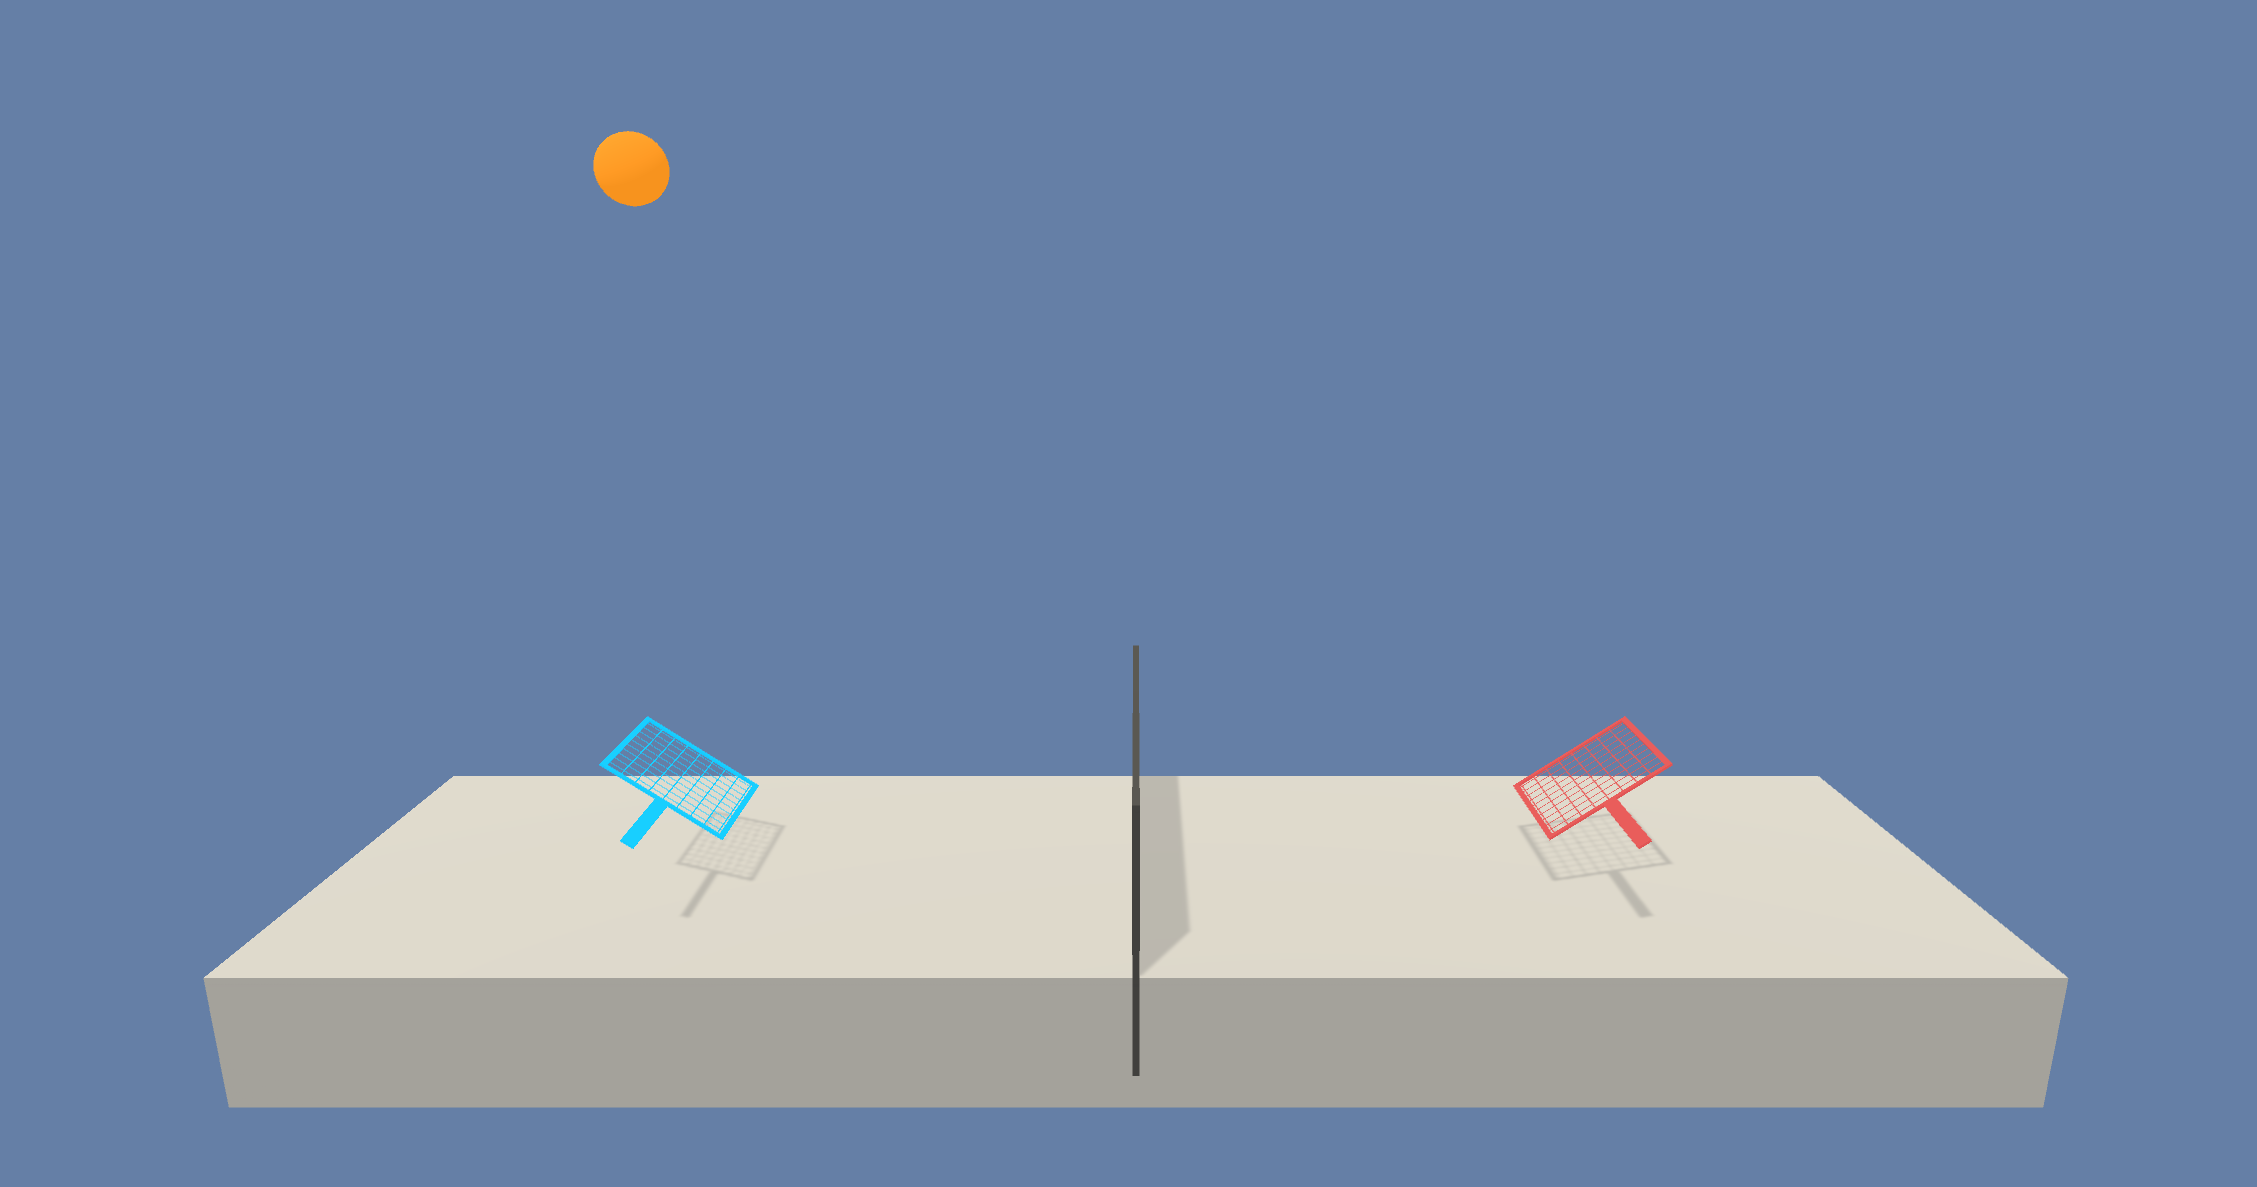
\includegraphics[scale=0.12]{tennis.png}
\caption{The environment}
\label{fig:tennis}
\end{figure}
This environment is a version of Unity ML-Agent Tennis environment, suitable to test reinforcement learning algorithms. Solving this continuous spaces environment will need the use Agent - Critic \cite{actcrit} method to approximate the best policy, in this case the use of Deep Deterministic Policy Gradient (DDPG) algorithm. 

\section{Environment}

The environment is an inertial plus gravity simulation of a ball and two players with represented by rackets. The goal is to keep the ball in the air as much time as possible following the regular tennis rules.
In this case, there are two agents and they learn by self playing.
The environment grants a positive reward of +0.1 when the agent is able to hit the ball over the net and -0.1 when the ball hits the player ground or go out of bound following the tennis rules \newline
The environment is considered solved when the average 100 rewards of of the average rewards collected by the twenty agents is bigger than 0.5.\newline
The action space is a 2 dimension vector corresponding to jump and going towards or against the net.\newline
Task is episodic and rewards are given during the episode.

\section{Algorithm}
The agent learns using an Actor - Critic \cite{ddpg} approach and a DDPG algorithm for estimate the value action function .\newline
This algorithm has two neural networks, one for the Actor and One for the Critic. 
The Actor tries to approximate the best policy in a deterministic way \newline.
Because the Agent is deterministic, noise has to be added to encourage the exploration.\newline
The policy network weights are updated using a policy gradient.\newline
The Critic gets the State and Action and returns the Q value, which is the action - value function (using DQN) approximated on the NN weights.\newline
\subsection{Neural networks architecture}
The Agent neural network used has the following architecture
\begin{table}[!htbp]
\center
\begin{tabular}{l|l|l|l|l}
Layer         & Neurons   & Type & Activation & Comment  \\
\hline
Input  &  8 &	&	& according to the space state dimension\\
Hidden & 256 &	Linear &	ReLU &\\	
Hidden & 256 &	Linear &	ReLU &\\ 	
Output &   1 &	Linear &	tanh & To get values on $[-1,1] \in R$ 
\end{tabular}
\end{table}

The Critic neural network used has the following architecture
\begin{table}[!htbp]
\center
\begin{tabular}{l|l|l|l|l}
Layer         & Neurons   & Type & Activation & Comment  \\
\hline
Input  &  8 &	&	& according to the space state dimension\\
Hidden &  512 + action vector size &	Linear &	ReLU &\\	
Hidden &  256 &	Linear &	ReLU &\\ 	
Output &   2 &	Linear &	ReLU & One for each action
\end{tabular}
\end{table}
\subsection{Hyperparameters}
The hyper parameters are the following:
\begin{table}[!htbp]
\center
\begin{tabular}{l|l|l}
Parameter         & Value   & Description  \\
\hline
$\gamma$ & 0.99 & Discount factor\\
$\tau$ &  0.001 & Soft-update ratio\\
Local network update interval every & 4 time steps &\\
Remote network update interval every & 4 time steps &\\
Replay buffer size & 1e6 &\\
Mini batch size & 128 &\\
$\epsilon$ - start & 1 & Start value\\
$\epsilon$ - min & 0.01 & Minimum value\\
$\epsilon$ - decay & 1e-6 & Decay rate\\
Learning rate for ACTOR & 1e-3 &\\
Learning rate for CRITIC: & 1e-4 & \\
L2 weight decay & 0 &\\
Learn every& 20 time-steps & \\
Number of learning passes& 10 & \\
Ornstein-Uhlenbeck noise $\sigma$ parameter & 0.2 & \\
Ornstein-Uhlenbeck noise $\theta$ parameter & 0.15 &
\end{tabular}
\end{table}
\section{Results}
The agent learns and achieve the goal on 100 episodes, but converges around episode 40, the environment is consider solved only averaging one hundred scores, therefore, the agent must wait.\newline

\subsection{Training}
The goal is to achieve an average score of 0.5 over last 100 episodes, with this hyper-parameters the agent solves the environment in 100 episodes with 1000 time-steps each.\newline
The algorithm waits to consider the environment solved, but will save the best model after every episode.\newline

Every episode consist in 1000 time steps maximum, after episode 80 the agent losses some precision, reducing the time steps does not help on this behaviour (but in other step) and can worth to research why this happens. The final result is not affected because the best model is saved along with the final model.\newline
The training history depiction is shown in Figure 2.

\begin{figure}[H]
\centering
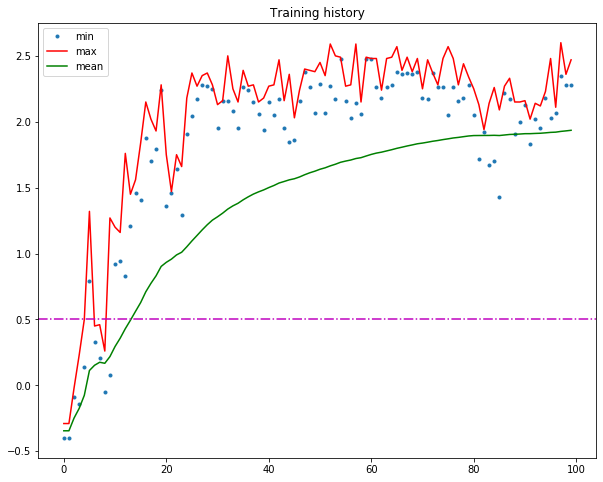
\includegraphics[scale=0.4]{training_1000.png}
\caption{Training, episodes vs rewards}
\label{fig:train_1000}
\end{figure}
\subsection{Playing}
The agent plays very well against itself and against a human user proving that the policy is reliable.

\section{Conclusions}
The agent learns very fast but play collaboratively only.\newline
The agent perform very well once trained, which is coherent with the learning graph.
\section{Future work}
This task is cooperative, so, the agent doesn't learn to compete, means,  play to win. The agent will perform well in preventing the ball to fall or go out of bounds, but wont play to win.\newline
To solve this the solution could be:
\begin{itemize}
\item Granting a rewards when the other player fails, if the environment cannot be modified, is enough to feed the last reward to the neural network.
\item Feeding the state of the the other player to the neural network
\end{itemize}

Check the possibility to consider the environment solved before, maybe some hyper parameter tuning can allow the agent to converge faster.\newline
\printbibliography
\end{document}